%%%%%%%%%%%%%%%%%%%%%%%%%%%%%%%%%%%%%%%%%%%%%%%%%%%%%%%%%%%%%%%%%%% 
%                                                                 %
%                            CHAPTER                              %
%                                                                 %
%%%%%%%%%%%%%%%%%%%%%%%%%%%%%%%%%%%%%%%%%%%%%%%%%%%%%%%%%%%%%%%%%%% 

\chapter{Related work}
\label{chapter:related_work}

In this chapter, we discuss the various technologies related to this thesis. We begin by discussing the semantic web and build from there to technologies used within its ecosystem like \acrshort{rdf}, \acrshort{sparql}, and mapping languages. We finish by discussing the current state of the art in updating or creating the original data source from a knowledge graph.

\section{Semantic Web}
Tim Berneers-Lee envisioned a version of the web that would also be understandable by machines, and thus the semantic web was born. It is not designed as a separate entity to the web, but instead as an extension, mostly hidden for normal humans. It is designed mostly with existing technologies like \acrshort{xml}(including HTML, being a superset of it), \acrshort{uri} and \acrshort{rdf}. Even ontologies, a key component of the semantic web, are not a new concept but rather co-opted from the field of philosophy. \citep{thesemanticweb}

\section{RDF}
\acrshort{rdf} was originally designed as a data model for metadata but has since been extended to be a general-purpose framework for graph data. RDF is a directed graph, where the nodes represent entities, and the edges represent relations between these entities. This graph is built up from triples, which connect a subject and an object using a predicate as shown in figure \ref{fig:rdf_triple}.

\begin{figure}
    \centering
    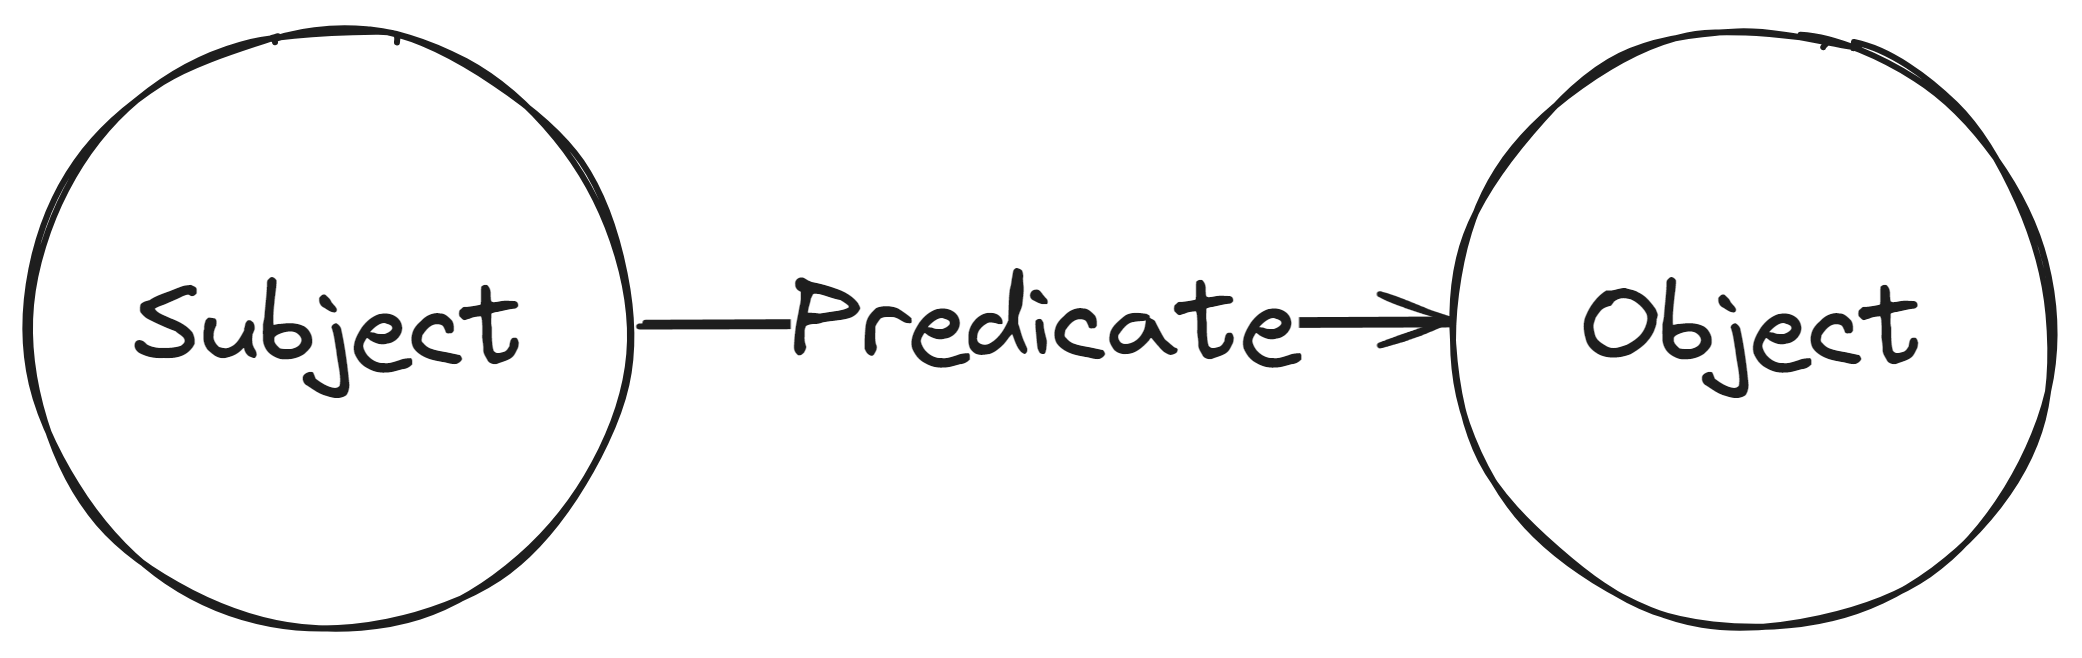
\includegraphics[width=0.5\textwidth]{Chapter2/SPO}
    \caption{An RDF triple}
    \label{fig:rdf_triple}
\end{figure}

The subject must always be an entity, which can either be represented by an \acrshort{uri} or be a blank node. The predicate must be an \acrshort{uri}, and the object can be either an \acrshort{uri}, a blank node, or a literal. \citep{rdfprimer}

\begin{figure}[]
    \begin{tabular}{lll}
        \textbf{Subject}             & \textbf{Predicate}           & \textbf{Object}                           \\
        http://example.com/De\_Nayer & https://schema.org/location  & http://example.com/Sint\_Katelijne\_Waver \\
        http://example.com/r0785695  & https://schema.org/givenName & ``Tijs"
    \end{tabular}
    \caption{Example of RDF triples}
    \label{fig:rdf_triples_table}
\end{figure}

An \acrshort{uri} is a unique identifier for a resource on the web. Unlike a normal \acrshort{url}, it does not have to point to a network location, but can also be used to identify a person, a location, a concept, etc. \citep{rdfprimer}. In \acrshort{rdf} the \acrshort{uri} is purely used for identifying resources. As such, unlike in HTML where certain conventions are expected, there are no conventions for \acrshortpl{uri} in \acrshort{rdf}. An example of this can be seen in figure \ref{fig:rdf_triples_table}, the example subjects share the same domain but this does not imply that they are closely related, or even related at all. \acrshortpl{uri} are extended to \acrshortpl{iri} to allow for a wider range of characters. Except for allowing Unicode characters, \acrshortpl{iri} are identical to \acrshortpl{uri} so little distinction is made between the two in this thesis.

A blank node is a node that is not identified by a \acrshort{uri}. It is used to represent an anonymous resource that can't be or has no reason to be uniquely identified. For example, the address of student r0785695 in figure \ref{fig:blank_node} is only pertinent to the student and thus does not need to be uniquely identified. A blank node is serialized as \texttt{\_:name}, where name is a unique identifier for the blank node. This identifier is only unique within the document, and thus can't be used to refer to the blank node from outside the document. \citep{rdfprimer}

\begin{figure}[]
    \begin{tabular}{lll}
        \textbf{Subject}    & \textbf{Predicate}   & \textbf{Object}                                     \\
        ex:student/r0785695 & schema:address       & \_:addrr0785695                                     \\
        \_:addrr0785695     & schema:postalCode    & "2800"\textasciicircum \textasciicircum xsd:integer \\
        \_:addrr0785695     & schema:streetAddress & "Gentsesteenweg XXXX"@nl
    \end{tabular}
    \caption{Example of a blank node and prefix notation}
    \label{fig:blank_node}
\end{figure}

A literal is a value, e.g. a string, integer, or date. This value can be typed, e.g. a string can be typed as a date, or untyped. A string can also have a language tag, which is used to indicate the language of the literal.

RDF is only a framework, and as such does not define any serialization syntax. There are however a few common serialization standards for example RDF/XML, Turtle, N-Triples, and JSON-LD.

\subsection{Turtle}
Turtle, or Terse RDF Triple Language, is a human-readable serialization format for \acrshort{rdf}. It is the most used serialization format for \acrshort{rdf}, and is used in many tools and specifications.
In its simplest form turtle consists of triple statements, sequences of subject-predicate-object separated by spaces and terminated by a dot. An example of this can be seen in listing \ref{lst:basic_turtle_example}. This is very verbose, but Turtle offers many features to make it more concise. Below is a list of some of these features and, if possible, how they can be used to make the example more concise.
\begin{itemize}
    \item \textbf{Prefix notation} allows us to shorten \acrshortpl{uri} by defining a prefix.
          \begin{itemize}
              \item Using \texttt{@prefix schema: <https://schema.org/>} allows us to shorten \break\texttt{https://schema.org/Person} to \texttt{schema:Person}
          \end{itemize}
    \item \textbf{Base prefix} allows us to shorten \acrshortpl{uri} by defining a base \acrshort{uri}.
          \begin{itemize}
              \item Using \texttt{@base <http://example.com/>} allows us to shorten \break\texttt{http://example.com/r0785695} to \texttt{r0785695}
          \end{itemize}
    \item \textbf{Predicate lists} allow us to shorten multiple triples with the same subject to a list of predicates.
          \begin{itemize}
              \item Our example only has two subjects, we can split their predicates with \texttt{;} instead of repeating the subject.
          \end{itemize}
    \item \textbf{Object lists} allow us to shorten multiple triples with the same subject and predicate to a list of objects.
          \begin{itemize}
              \item \texttt{r0785695} is both a Person and a Student, so we can split the objects with \texttt{,} instead of repeating the subject and predicate.
          \end{itemize}
    \item \textbf{Literals} allow identifying values, e.g. strings, integers, dates, etc. with a datatype or language tag.
    \item \textbf{Blank nodes} allow us to define anonymous resources by using the \texttt{\_:} prefix.
          \begin{itemize}
              \item The address of \texttt{r0785695} is only relevant to \texttt{r0785695}, so we can define it as a blank node instead of using a \acrshort{uri}, this shortens \texttt{<http://example.com/addrr0785695>} to \texttt{\_:addrr0785695}. While not exactly the same, functionally it is equivalent as we do not expect addresses to be addressed outside of the context of a person.
          \end{itemize}
    \item \textbf{Unlabeled blank nodes} allow us to define anonymous resources without a unique identifier by using the [] notation instead of \texttt{\_:name}.
          \begin {itemize}
    \item As we do not need to refer to \texttt{\_:addrr0785695} from outside \texttt{r0785695}, we can use an unlabeled blank node and include it in \texttt{r0785695} instead of a labeled blank node.
\end{itemize}
\item \textbf{Collections} allow us to define a list of blank nodes by using the () notation.
\end{itemize}
The example in listing \ref{lst:basic_turtle_example} can be rewritten using these features, as shown in listing \ref{lst:basic_turtle_example_concise}.


\begin{lstlisting}[caption={Basic naive turtle document}, label={lst:basic_turtle_example}, captionpos=b, breaklines=true, basicstyle=\small]
    <http://example.com/r0785695> <http://www.w3.org/1999/02/22-rdf-syntax-ns#type> <http://schema.org/Person> .
    <http://example.com/r0785695> <http://www.w3.org/1999/02/22-rdf-syntax-ns#type> <http://schema.org/Student> .
    <http://example.com/r0785695> <http://schema.org/givenName> "Tijs" .
    <http://example.com/r0785695> <http://schema.org/familyName> "Van Kampen" .
    <http://example.com/r0785695> <http://schema.org/address> <http://example.com/addrr0785695> .
    <http://example.com/addrr0785695> <http://schema.org/postalCode> "2800"^^<http://www.w3.org/2001/XMLSchema#integer> .
    <http://example.com/addrr0785695> <http://www.w3.org/1999/02/22-rdf-syntax-ns#type> <http://schema.org/PostalAddress> .
    <http://example.com/addrr0785695> <http://schema.org/streetAddress> "Gentsesteenweg XXXX"@nl .
    <http://example.com/addrr0785695> <http://schema.org/addressCountry> "Belgium" .
\end{lstlisting}

\begin{lstlisting}[caption={Basic turtle document using turtle features}, label={lst:basic_turtle_example_concise}, captionpos=b, breaklines=true]
    @prefix schema: <https://schema.org/> .
    @prefix xsd: <http://www.w3.org/2001/XMLSchema#> .
    @base <http://example.com/> .
    <r0785695> a schema:Person, schema:Student ;
        schema:givenName "Tijs" ;
        schema:familyName "Van Kampen" ;
        schema:address [
            a schema:PostalAddress ;
            schema:postalCode "2800"^^xsd:integer ;
            schema:streetAddress "Gentsesteenweg XXXX"@nl ;
            schema:addressCountry "Belgium"
        ] .
\end{lstlisting}


\section{SPARQL}
\acrfull{sparql} is the \acrshort{w3c} standard query language for \acrshort{rdf}. It is the main way to query \acrshort{rdf} data and shows many similarities to SQL. \acrshort{sparql} queries mostly consist of a pattern of triples, which are matched against the \acrshort{rdf} graph, a basic example can be found in listing \ref{lst:sparql_select_query}. Querying is very feature-rich, with support for aggregation, subqueries, negation, regex, string manipulation, etc. It also supports different return types, federated queries, entailment, etc \citep{SPARQL1.1QL}. Aside from the query protocol it also defines the graph store protocol, which can be used to manipulate graph databases directly \citep{SPARQL1.1}.

\begin{lstlisting}[language=SPARQL, caption={Example of a basic \acrshort{sparql} SELECT query}, label={lst:sparql_select_query}, captionpos=b]
    PREFIX schema: <https://schema.org/>
    SELECT ?name ?address
    WHERE {
        ?student schema:givenName ?name .
        ?student schema:address ?address .
    }
\end{lstlisting}

\section{Mapping languages}
Mapping languages are used to define a mapping between a source and a target. The target in the context of linked data is of course \acrshort{rdf}, with the source being any structured data source. Some mapping languages exist for a single source, e.g. \acrfull{r2rml} for relational databases, \acrfull{xsparql} for \acrshort{xml}, etc. Others are more general purpose, e.g. \acrfull{rml} and \acrfull{d2rml}.
We will discuss both \acrshort{r2rml} and \acrshort{rml} in more detail, as one extends the other. \acrshort{rml} we will discuss because it is one of the more feature-rich general mapping languages, and it is the mapping language we will use in our implementation. \acrshort{r2rml} we discuss because it is the most widely used mapping language, as it supports virtualization \textit{ontop} of databases. % ontop is a tool that allows virtualization
Most \acrshort{rml} implementations also support \acrshort{r2rml}, as \acrshort{rml} is a nearly superset of \acrshort{r2rml}.

\subsection{\acrshort{r2rml}}
\acrfull{r2rml} is a mapping language for mapping relational databases to \acrshort{rdf}. As opposed to \acrfull{dm}, which results in a direct mapping from the relational database to \acrshort{rdf} without any changes to structure or naming, \acrshort{r2rml} allows for more flexibility. R2RML mappings consist of zero or more TriplesMaps, which are used to map a table to \acrshort{rdf}. A TriplesMap consists of a logical table, a subject map, and one or more \acrfullpl{pom}.

The logical table is used to define the table that is being mapped, with each row in the table being mapped to a subject and its corresponding \acrshortpl{pom}. It is possible to create a view of a table by using a SQL query, and then map this view. This allows for more complex mappings, e.g. mapping a join of two tables or a computed column.
% Could add this, but as we don't actually support R2RML in our implementation for now this is not really relevant
% An example of this can be seen in listing \ref{lst:r2rml_mapping_view}.

% \begin{lstlisting}[caption={Example of an \acrshort{r2rml} mapping with a view. Snippet from \citep{r2rml}}, label={lst:r2rml_mapping_view}, captionpos=b] 
%     <#TriplesMap1>
%     rr:logicalTable [ rr:sqlQuery """
%         SELECT EMP.*, (CASE JOB
%             WHEN 'CLERK' THEN 'general-office'
%             WHEN 'NIGHTGUARD' THEN 'security'
%             WHEN 'ENGINEER' THEN 'engineering'
%         END) ROLE FROM EMP
%         """ ];
%     rr:subjectMap [
%         rr:template "http://data.example.com/employee/{EMPNO}";
%     ];
%     rr:predicateObjectMap [
%         rr:predicate ex:role;
%         rr:objectMap [ rr:template "http://data.example.com/roles/{ROLE}" ];
%     ].
% \end{lstlisting}

Each of the SubjectMap, PredicateMap, ObjectMap, (and GraphMap) is a subclass of TermMap, which is a function that generates an \acrshort{rdf} term. The map type can be constant, template, or column. The resulting term is then used as the subject, predicate, object, or graph of the triple. The termType of the map determines the type of the term, which can be \acrshort{iri}, blank node, or literal. If the termType is literal, optionally the datatype or language can be added. Following the \acrshort{rdf} specification, not all combinations of termType and map are possible, this is shown in table \ref{tab:termType_map_combinations}. The object map has an additional subclass, a reference object map, in which we refer to another TriplesMap. Using a reference map we can map a foreign key to the subject of another TriplesMap, with a join condition. \citep{r2rml}

\begin{table}[h]
    \begin{tabular}{|l|l|l|l|l|}
        \hline
        \textbf{TermType} & \textbf{Subject} & \textbf{Predicate} & \textbf{Object} & \textbf{Graph} \\ \hline
        IRI               & \cmark           & \cmark             & \cmark          & \cmark         \\ \hline
        Blank node        & \cmark           & \xmark             & \cmark          & \cmark         \\ \hline
        Literal           & \xmark           & \xmark             & \cmark          & \xmark         \\ \hline
    \end{tabular}
    \caption{Possible combinations of TermType and Map type}
    \label{tab:termType_map_combinations}
\end{table}

A constant value is a fixed value, e.g. a \acrshort{uri} or a string. A template is a string with placeholders, which are replaced by values from the logical row. A column is the value of a column in the logical row.

\begin{lstlisting}[language=XML, caption={Example of an \acrshort{r2rml} mapping}, label={lst:r2rml_mapping}, captionpos=b]
@prefix rr: <http://www.w3.org/ns/r2rml#>.
@prefix ex: <http://example.com/ns#>.

<#TriplesMap1>
    rr:logicalTable [ rr:tableName "EMP" ];
    rr:subjectMap [
        rr:template "http://data.example.com/employee/{EMPNO}";
        rr:class ex:Employee;
    ];
    rr:predicateObjectMap [
        rr:predicate ex:id;
        rr:objectMap [ rr:column "EMPNO"; rr:datatype xsd:positiveInteger ].
    ].
\end{lstlisting}

\subsection{\acrshort{rml}}
\acrfull{rml} is a mapping language for mapping any (semi-)structured data source to \acrshort{rdf}. It is a generalization of \acrshort{r2rml} and as such supports all the features of \acrshort{r2rml}. It extends \acrshort{r2rml} by extending database-specific features to make them more general. The differences in usage can be seen in table \ref{tab:r2rml_rml_differences}. \citep{rml}

\begin{table}[]
    \begin{tabular}{|ll|ll|}
        \hline
        \multicolumn{2}{|c|}{R2RML}         & \multicolumn{2}{c|}{RML}                                                           \\ \hline
        Logical Table (relational database) & rr:logicalTable          & Logical Source               & rml:logicalSource        \\ \hline
        Table Name                          & rr:tablename             & URI (pointing to the source) & rml:source               \\ \hline
        column                              & rr:column                & reference                    & rml:reference            \\ \hline
        (SQL)                               & rr:SQLQuery              & Reference Formulation        & rml:referenceFormulation \\ \hline
        per row iteration                   &                          & defined iterator             & rml:iterator             \\ \hline
    \end{tabular}
    \caption{Differences between \acrshort{r2rml} and \acrshort{rml}}
    \label{tab:r2rml_rml_differences}
\end{table}

\acrshort{rml} uses the same structure as \acrshort{r2rml}, with TriplesMaps consisting of a logical source, a subject map, and zero or more \acrshortpl{pom}. The changes it has all relate to the logical source. Whereas in \acrshort{r2rml} the source is always a database, from which we select a table or view, in \acrshort{rml} the source can be one of many different source types like \acrshort{xml}, \acrshort{json}, \acrshort{csv}, etc. Where in \acrshort{r2rml} we simply iterate over the rows of a table, in \acrshort{rml} we can have a source without an explicit iteration pattern, and as such we need to define an iterator.

% \section{if meaningful: provenance}
% provenance could be interesting but is not mainstream enough to use on a larger scale. (-yet? Maybe in future work add a reference)

\section{State of the art}
The state of the art in updating or creating the data source from a knowledge graph can be split in two categories, depending on the methodology used. The first methodology applies to virtualization, where the data is exposed as a virtual knowledge graph over the source data. The other methodology is for materialized knowledge graphs, where the knowledge graph is created as a file that can be loaded into a triple store. We will discuss the state of the art in both methodologies, concluding with the relevance of this work.

\subsection{Virtualization}
Virtualization is the process of exposing a virtual knowledge graph over the source data. This virtual knowledge graph can be queried as if it were a real knowledge graph. To achieve this mappings are used to translate queries over the knowledge graph to queries over the source data.

This is most commonly used to expose a database as a virtual knowledge graph. This way an organization can expose a knowledge graph without having to completely transition to a new system. Most implementations of virtualization layers are read-only though, as the translation of SELECT queries is relatively easy but translating INSERT, DELETE or DELETE/INSERT (update) queries is much less straightforward, or even impossible in many cases. Though propagating changes trough the virtualization layer to the source data could be a big part of the linked data lifecycle, related work on this is scarce. In both "SPARQL Update queries over R2RML mapped data sources" \citep{unbehauen-k-2017--sparqlUpdate} and "Practical Update Management in Ontology-Based Data Access" \citep{practical_update_management_in_ontology_based_data_access} the authors propose a similar way of handling updates. Compatible updates are propagated to the source data, while incompatible updates are held in an 'overflow' triple store. Further changes may make the incompatible updates compatible, at which point they too are propagated to the source data. Larger changes affecting the general structure of the data are not stored, but instead the mapping is updated to reflect the new structure. The handling of updates is shown in figure \ref{fig:virtualization_update}.

\begin{figure}
    \centering
    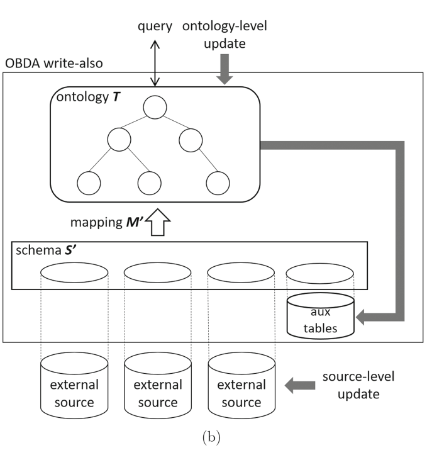
\includegraphics[width=0.6\textwidth]{Chapter2/Write-also_ODBA_architecture.png}
    \caption{Propagating changes in a virtualization layer}
    \label{fig:virtualization_update}
\end{figure}

\subsection{Materialization}
Materialization is the process of creating a knowledge graph as a file that can be loaded into a triple store. The knowledge graph is then loaded into a dedicated triple store for querying. This method benefits from increased performance, at the cost of having the knowledge graph not in sync with the source data.

Materialization allows for a wider range of source formats, as the knowledge graph can be created from any structured data source. This is especially useful when the source data is not easily queryable, e.g. when the source data is a \acrshort{csv}, \acrshort{xml}, or \acrshort{json} file. For knowledge graphs created from structured data sources, use cases exist for propagating changes back to the original data source. This is not done using a direct update (as the source data is not directly connected to the knowledge graph), but by creating a new version of the source data. This process is called lowering. Below we discuss some of the state of the art in lowering.

\subsubsection{\acrshort*{xsparql}}
\acrshort{xsparql} is a mapping language that allows for the transformation of \acrshort{xml} to and back from \acrshort{rdf}. It expands XQUERY with SPARQL-like syntax, structure and features. Its predecessors would do lifting by querying the source \acrshort{xml} using \acrshort{xquery} to transform it into the \acrshort{xml} serialization of \acrshort{rdf}, while lowering was done using XSLT to do the inverse. Using its combined vocabulary \acrshort{xsparql} simplifies lifting and lowering, using a single language for both and having the ability to target the turtle serialization \citep{xsparql}. An example lifting and lowering query can be found in listing \ref{lst:xsparql_lifting} and listing \ref{lst:xsparql_lowering} respectively.

\begin{lstlisting}[caption={Example of \acrshort{xsparql} lifting}, label={lst:xsparql_lifting}, captionpos=b, basicstyle=\small]
declare namespace foaf="http://xmlns.com/foaf/0.1/";
declare namespace rdf="http://www.w3.org/1999/02/22-rdf-syntax-ns#";
let $persons := //*[@name or ../knows]
return

for $p in $persons
let $n := if( $p[@name] )
            then $p/@name else $p
let $id := count($p/preceding::*)
            +count($p/ancestor::*)
where
    not(exists($p/following::*[
        @name=$n or data(.)=$n]))
construct {
    [*_:b{$id} a foaf:Person;*]
                [*foaf:name {data($n)}.*]
    {
        for $k in $persons
        let $kn := if( $k[@name] )
                    then $k/@name else $k
        let $kid := count($k/preceding::*)
                    +count($k/ancestor::*)
        where
            $kn = data(//*[@name=$n]/knows) and
            not(exists($kn/../following::*[
                @name=$kn or data(.)=$kn]))
        construct {
        [*_:b{$id} foaf:knows _:b{$kid}.*]
        [*_:b{$kid} a foaf:Person.*]
        }
    }
}
\end{lstlisting}

\begin{lstlisting}[caption={Example of \acrshort{xsparql} lowering}, label={lst:xsparql_lowering}, captionpos=b, basicstyle=\small]
<relations>{
    for $Person $Name from <relations.rdf>
    where {$Person foaf:name $Name}
    order by $Name
    return
        <person name="{$Name}">{
            for $FName from <relations.rdf>
            where {
                $Person foaf:knows $Friend.
                $Person foaf:name $Name.
                $Friend foaf:name $Fname. }
            return
            <knows>{$FName}</knows>
        }</person>
}</relations>
\end{lstlisting}


\subsubsection{POSER: A Semantic Payload Lowering Service \citep{poser}}
POSER(Payload lOwering SERvice) is a service that lowers \acrshort{rdf} to \acrshort{json}. To achieve this a mapping is created in two parts: first the source patterns are defined from which to extract the data, then the json structure is defined. The mapping is written in turtle, using a custom json ontology describing the json structure. A proof of concept implementation was made, but never got out of the prototype phase. It also only handles direct literal types, more complex composite values that are generated from templates are not supported. An example mapping is shown in listing \ref{lst:poser_mapping}.

\begin{lstlisting}[caption={Example of a POSER mapping}, label={lst:poser_mapping}, captionpos=b, basicstyle=\small]
@prefix ctd: <http://connectd.api/> .
@prefix onto: <http://ontodm.com/OntoDT#> .
@prefix iots: <http://iotschema.org/> .
@prefix json: <http://some.json.ontology/> .
@prefix xsd: <http://www.w3.org/2001/XMLSchema#> .
@prefix time: <https://www.w3.org/TR/2020/CR-owl-time-20200326/> .

# Which inputs to expect and to start mapping from
json:InputDataType {
    json:EntryPoint a iots:TimeSeries;
        iots:providesTemperatureData iots:TemperatureData;
        iots:providesTimeData iots:TimeData .

    iots:TemperatureData iots:numberDataType iots:Number .
    iots:TimeData  time:dateTime iots:Number .
}

#Semantic description of the json objects to be found in the expected API

json:ApiDescription {
    ctd:JsonModel json:hasRoot ctd:Node .

    ctd:TemperatureValue a json:Number ;
        json:key "value"^^xsd:string ;
        json:dataType iots:TemperatureData .

    ctd:TimeStamp a json:String ;
        json:key "timestamp"^^xsd:string ;
        json:dataType iots:TimeData .

    ctd:Node a json:Object;
        json:key "node"^^xsd:string ;
        json:value ctd:TimeStamp, ctd:TemperatureValue ;
        json:dataType iots:TimeSeries .

    ctd:Edges a json:Array	;
        json:key "edges"^^xsd:string ;
        json:value ctd:Node .
}
\end{lstlisting}

\subsection{Relevance}
As shown in this section the state of the art in updating the source in virtualization is pretty mature, only limited by fundamental limitations. It is however limited to databases. To work with other (semi-)structured data sources materialization is needed. For materialization the state of the art is much more limited. Though methods exist to lower \acrshort{rdf} to other formats, each method is intimately linked to a source type. The mappings are also unidirectional, even \acrshort{xsparql} which offers both lifting and lowering requires a separate mapping for each. 

Our work expands RML, which can map from any structured data source to \acrshort{rdf}, with the ability to lower the \acrshort{rdf} back to the original source. We use a single mapping to do both lifting and lowering, as information on where to find the data during lifting can also be used to find where to put the data during lowering. This makes our work unique in the field of lowering \acrshort{rdf} to other formats.